\setcounter{chapter}{3}
\chapter{System Performance} \label{ch:performance}

Spectral efficiency is a key performance metric for multicarrier systems such as OFDM, as it quantifies how efficiently the available bandwidth is used to transmit useful information. It is formally defined as the number of successfully transmitted information bits per second per Hertz (bit/s/Hz). In this project, this metric serves to evaluate the trade-offs introduced by modulation order, coding rates, frame structure, and the various overheads inherent to the OFDM physical layer.

\section{Analytical Framework}

For the implemented OFDM system, the spectral efficiency $\eta$ is derived by accounting for the modulation order, coding gains, and structural overheads. The analytical expression is formulated as follows:

\begin{equation} \label{eq:spectral_efficiency_full}
    \eta = \mathrm{BPS} \cdot R_{\mathrm{FEC}} \cdot \underbrace{\frac{N_{\mathrm{data}}}{N_{\mathrm{carr}}}}_{\text{Subcarrier use}} \cdot \underbrace{\frac{N_{\mathrm{carr}}}{N_{\mathrm{carr}} + N_{\mathrm{cp}}}}_{\text{Guard interval}} \cdot \underbrace{\frac{N_{\mathrm{data\_sym}}}{N_{\mathrm{data\_sym}} + N_{\mathrm{training\_sym}}}}_{\text{Protocol overhead}} \eqend
\end{equation}

In this expression, $\mathrm{BPS}$ denotes the bits per symbol, $R_{\mathrm{FEC}}$ is the forward error correction rate, and the subsequent ratios represent the losses due to unused edge subcarriers, the cyclic prefix (CP), and the training symbols required for synchronization and channel estimation.

\section{Spectral Efficiency Trends and Trade-offs}

The efficiency of the system is sensitive to several design parameters, each presenting a fundamental compromise between throughput and link robustness.

\begin{remark}[Modulation and Bandwidth]
    Increasing the modulation order grows spectral efficiency logarithmically; however, higher-order constellations require significantly higher SNR to maintain acceptable bit error rates in noisy acoustic channels. Conversely, while increasing the occupied bandwidth scales the achievable data rate, the spectral efficiency remains unchanged, as the number of transmitted bits per Hertz is a property of the multicarrier structure itself.
\end{remark}

\begin{figure}[!ht]
    \ffigbox[\FBwidth]{%
        \begin{tabular}{cc}
            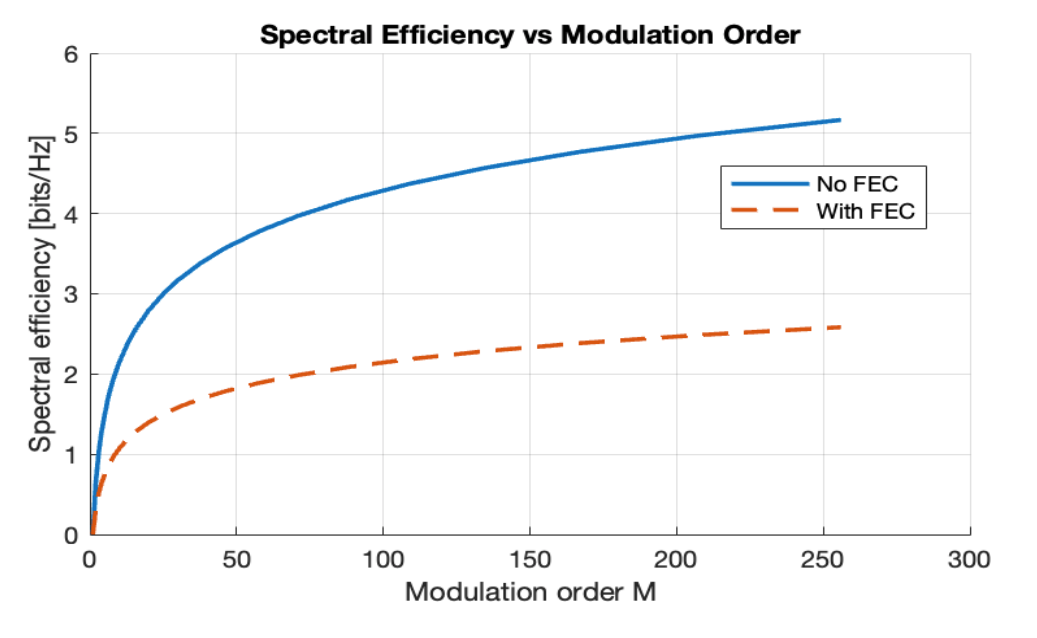
\includegraphics[width=0.45\textwidth]{figures/chap4_performance/Spectral_Efficiency_vs_Modulation_Order.png} & 
            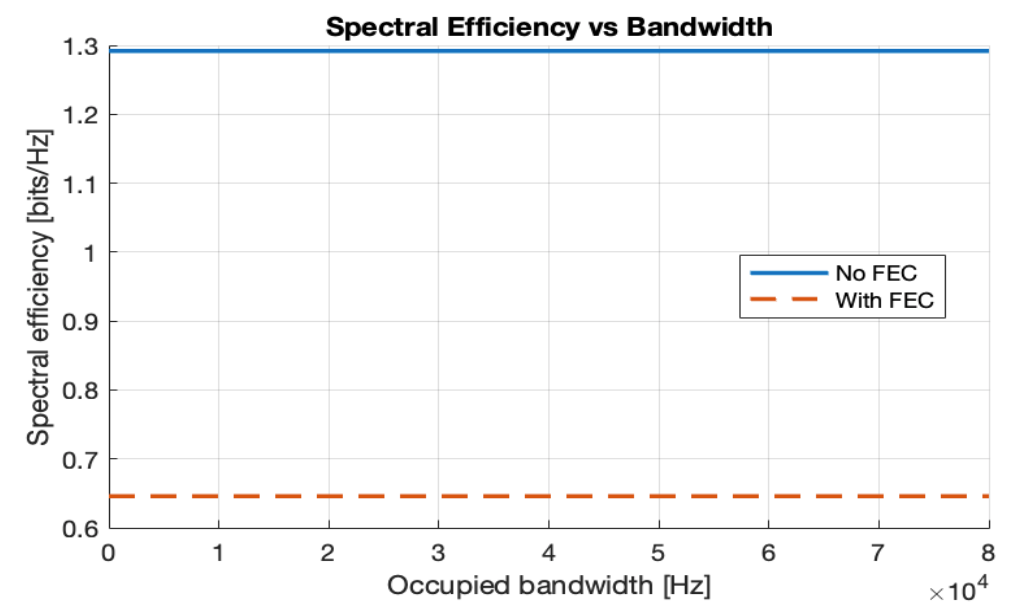
\includegraphics[width=0.45\textwidth]{figures/chap4_performance/Spectral_Efficiency_vs_Bandwidth.png} \\
        \end{tabular}
    }{%
        \caption[Modulation and Bandwidth Trends]{%
            (Left) Logarithmic growth of $\eta$ with modulation order. (Right) Constant spectral efficiency across varying bandwidths, illustrating the inherent behavior of multicarrier systems.
        }%
        \label{fig:eta_trends_basic}%
    }
\end{figure}

The temporal and frequency overheads also dictate the system's performance limits. Increasing the number of subcarriers $N_{\mathrm{carr}}$ improves efficiency by amortizing fixed overheads, though this gain saturates as the relative impact of unused carriers becomes negligible. In the time domain, the cyclic prefix is essential to preserve orthogonality in multipath environments, but it introduces a linear reduction in $\eta$ as its length $N_{\mathrm{cp}}$ increases.



\begin{figure}[!ht]
    \ffigbox[\FBwidth]{%
        \begin{tabular}{cc}
            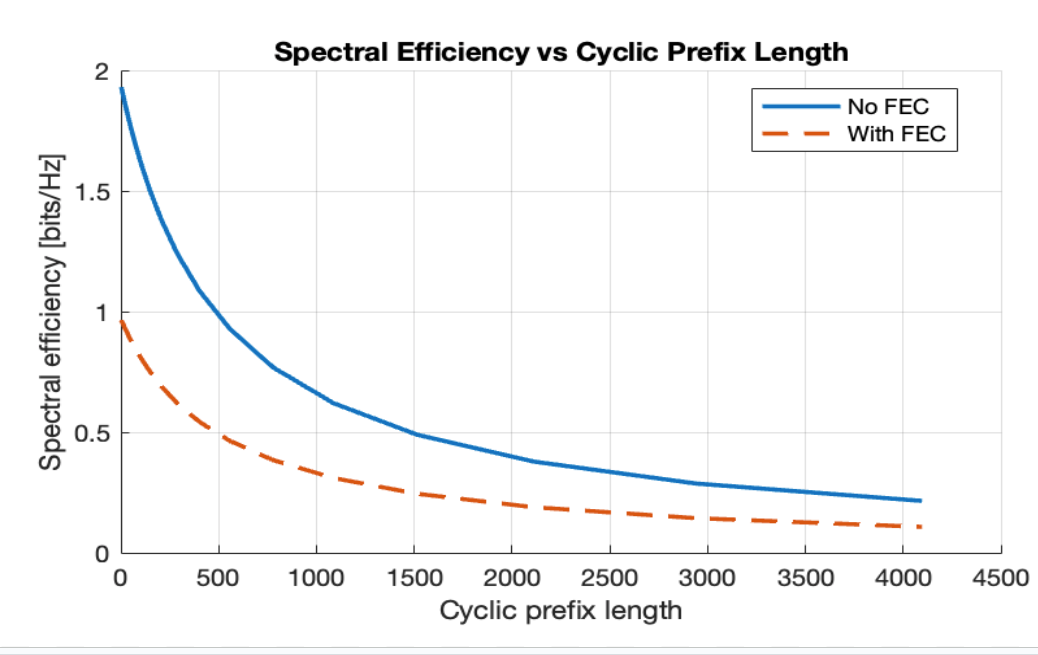
\includegraphics[width=0.45\textwidth]{figures/chap4_performance/Spectral_Efficiency_vs_Cyclic_Prefix_Length.png} & 
            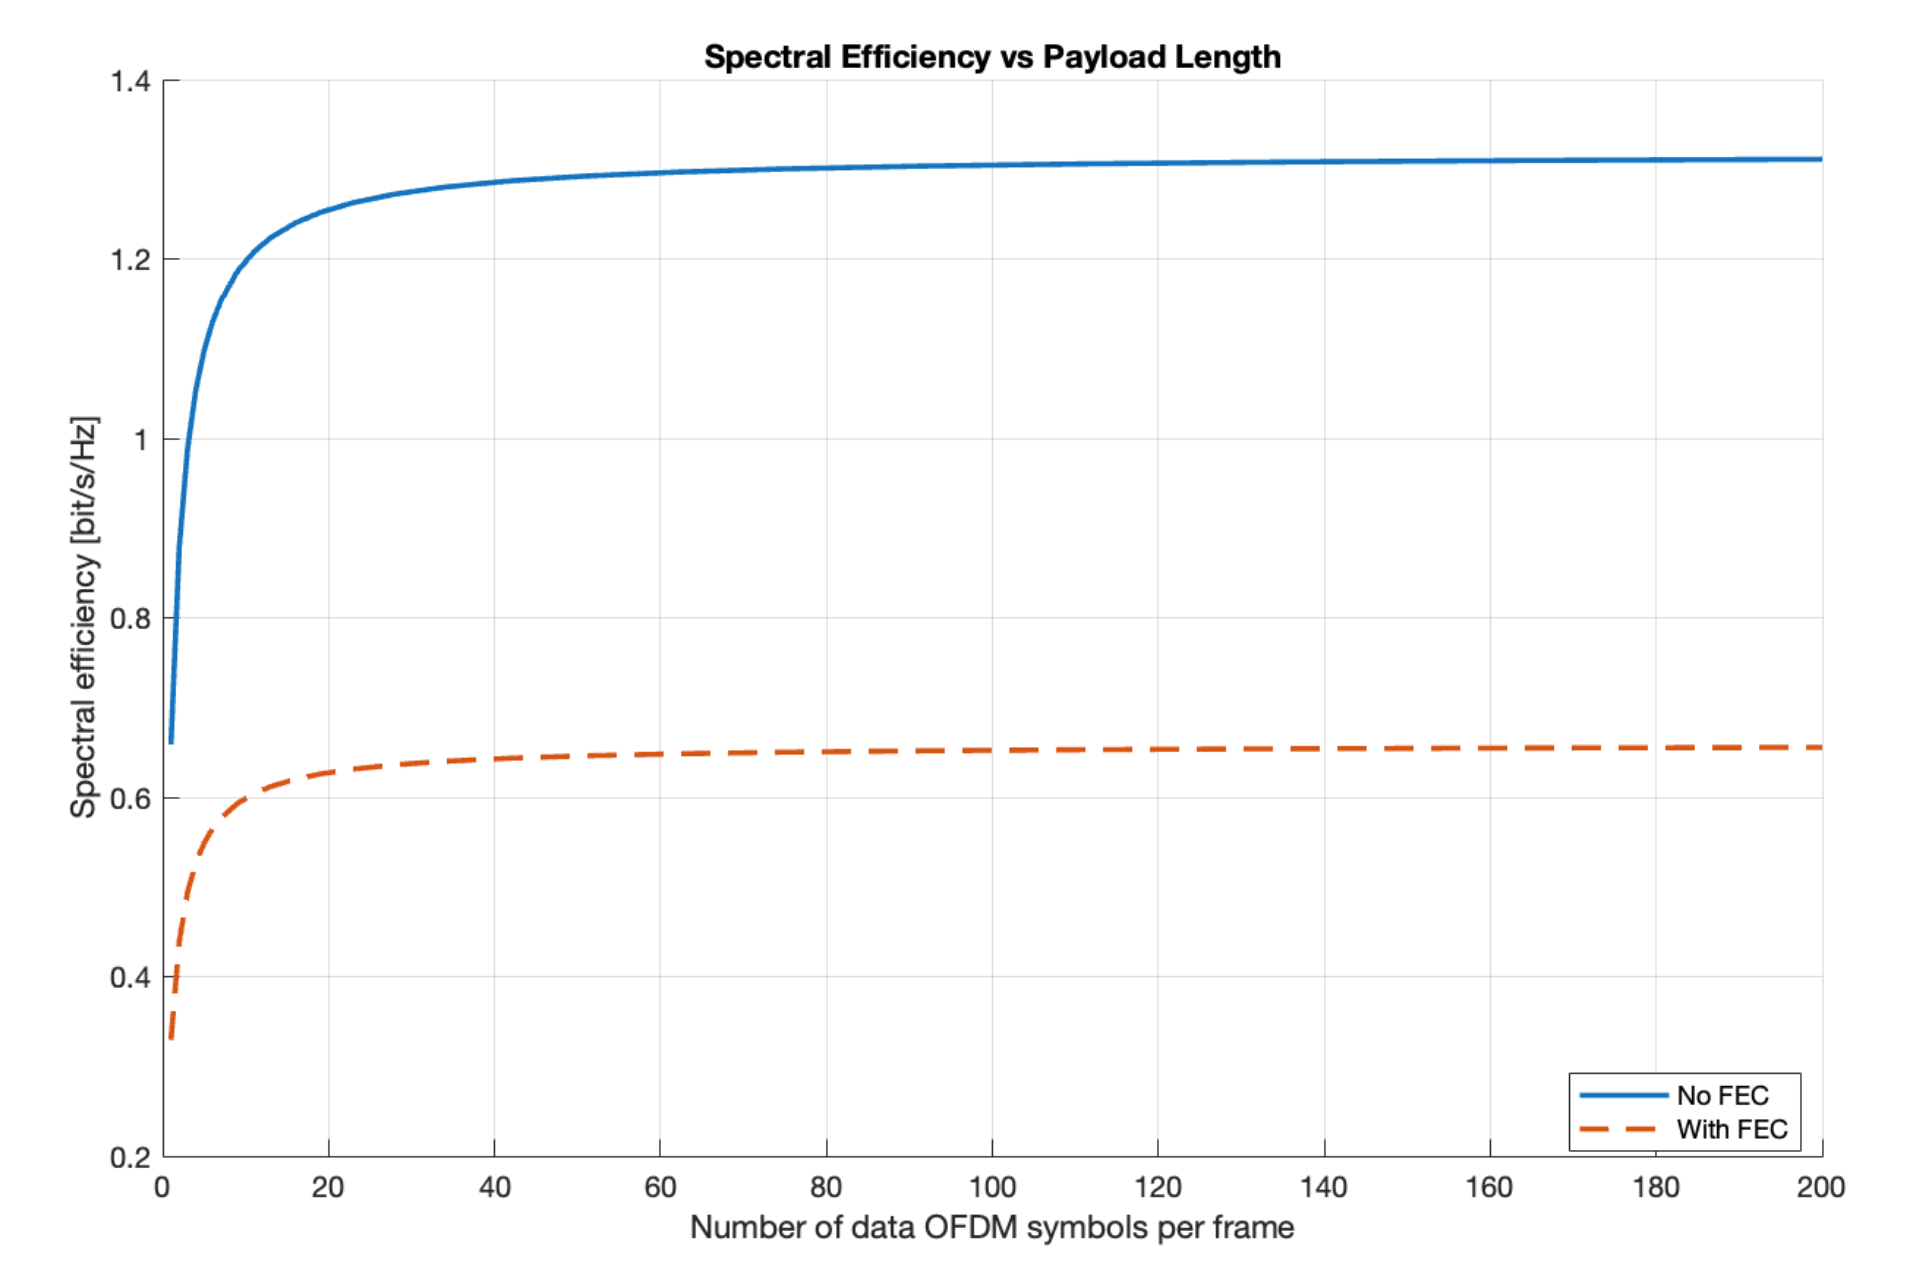
\includegraphics[width=0.45\textwidth]{figures/chap4_performance/Spectral_Efficiency_vs_Payload_Length.png} \\
        \end{tabular}
    }{%
        \caption[Temporal Overhead Impact]{%
            Effect of the cyclic prefix length and payload duration on efficiency. Longer payloads amortize the training symbol overhead, allowing $\eta$ to converge toward its theoretical upper bound.
        }%
        \label{fig:eta_overhead_trends}%
    }
\end{figure}

\begin{Note}[Amortization of Training Symbols]
    Training symbols are indispensable for synchronization, yet they reduce the fraction of useful data. As payload length increases, this overhead is amortized, motivating the use of long frames whenever the acoustic channel remains stationary.
\end{Note}

\section{Summary}

The spectral efficiency analysis highlights the fundamental design choices of the project. While higher modulation orders and larger payloads improve the bit/s/Hz ratio, the environmental constraints of the Rolex Learning Center—specifically multipath dispersion and noise—necessitate the use of cyclic prefixes and FEC. The final system parameters represent a calculated balance, ensuring reliable transmission at a sustainable information density.